Using the "Penn World Tables v. 9.0"\footnote{Downloadable from \url{https://www.rug.nl/ggdc/productivity/pwt/}} I analyze the development in the logarithm of real GDP per capita (at 2011 national prices) from 1950-2014 for Spain, (Western) Germany, and Denmark\footnote{Before taking the log, the Danish Kroner (DKK) is transformed to Euros by multiplication with 7.46038 which is the central exchange rate at which the DKK is pegged to the Euro within a tiny 2.5\% band, according to the \href{https://en.wikipedia.org/wiki/European_Exchange_Rate_Mechanism}{European Exchange Rate Mechanism (ERM)}.}.
\textbf{\textit{\begin{itemize}
  \item[a)] Plot the time series
\end{itemize}}}\noindent
From figure \ref{fig:23a} below it is obvious that the series for actual values of log GDP are not stationary while the transformed series, namely the first differences might be. Thus we will work with theese series instead.
\begin{figure}[H]
  \caption{Time series and first differences of log real GDP/capita}
  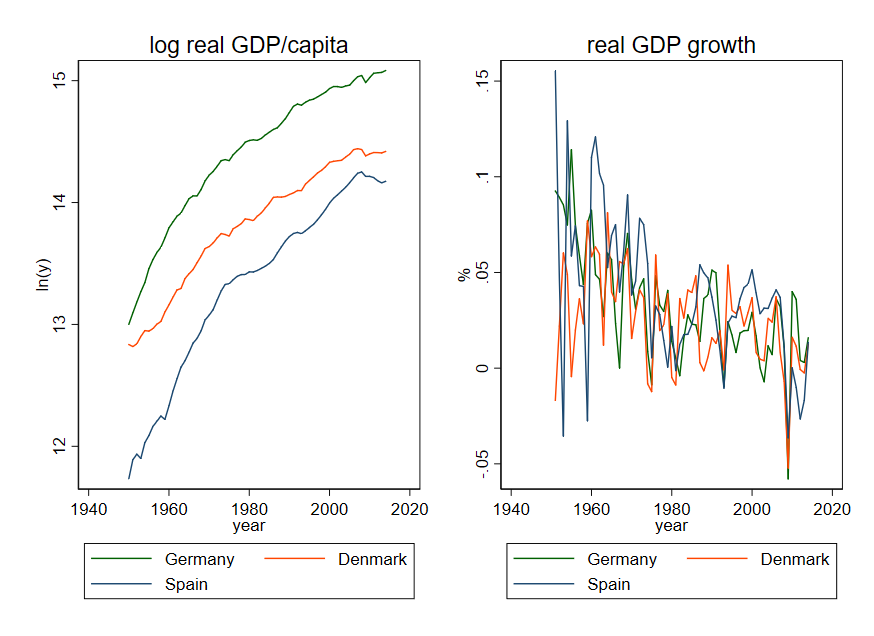
\includegraphics[width= \textwidth]{03_figures/fig23a}
  \label{fig:23a}
  \vspace{-1cm}
\end{figure}
However, the much higher growth rates in the 50s and 60s does raise the question of functional form even for the transformed processes of \nth{1} order. Is there a negative trend or a level shift? Also business cycles and especially negative shocks are evident. All three countries experience negative growth due to the busts in 1993 and 2009. Furthermore Denmark is hit significantly by the oil crisis in 1974-75 and Germany in 1975. Denmark also starts the 80s with negative growth rates due to the recession, while Germany again only experience detraction for one year in 1982 and again in 2003. The negative shock also shows persistence in Denmark in 2008-2009, even more so in Spain with detraction through 2011-13.
\textbf{\textit{\begin{itemize}
  \item[b)] Identification: using autocorrelation and partial autocorrelation functions, identify the orders of the ARIMA model. Compute both the numerical and graphical autocorrelation functions (including confidence bands)
\end{itemize}}}\noindent
The ACFs and PACFs in figure \ref{fig:23b} below show first of all that we do not need to worry about unit roots as none of the lags have an autocorrelation coefficient above $0.6$.

The GDP growth of Germany show signs of autocorrelation for up to 14 lags in the numerical correlogram and in the partial autocorrelation for lag 1, 3-4, 6-7, 9, as well as with several 16+ lags. The high number of lags in both the ACF and PACF suggests that German log real GDP can be approximated by an ARIMA(p,1,q) model. The graphical representation with the confidence bands however is more consistent with 4 ACF lags and 4 PACF lags, thus suggesting an ARIMA(4,1,4) model. However I choose to follow the Parsimonious principle of estimating the more simple model, thus, my more cautious suggestion would be an ARIMA(1,1,4) model as the coefficient of the second PACF lag is close to zero, well-knowing that we do loose information as lag 3 and 4 that both are clearly significant.
\begin{figure}[H]
  \caption{ACF and PACF of the first differences of log real GDP}
  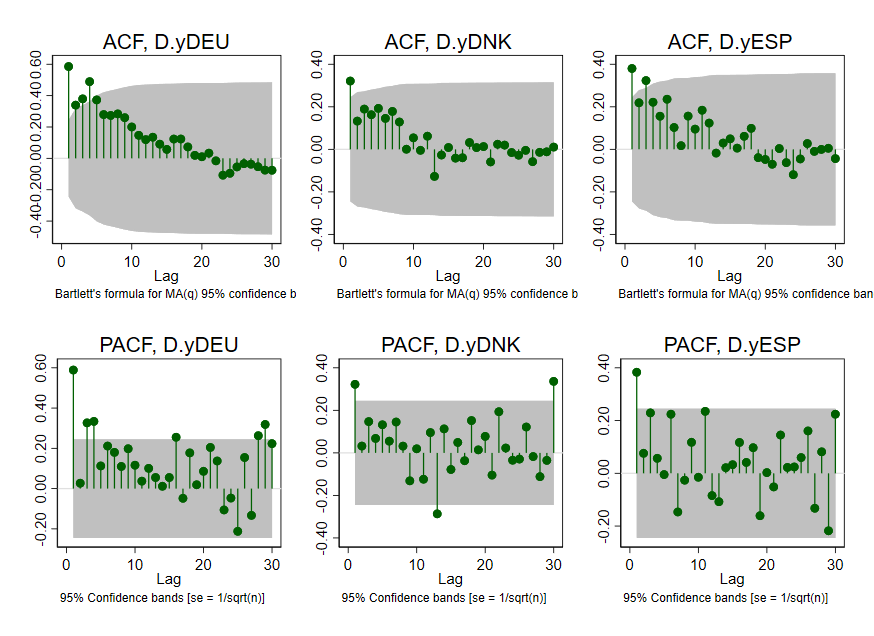
\includegraphics[width= \textwidth]{03_figures/fig23b}
  \label{fig:23b}
  \vspace{-1cm}
\end{figure}
While the graphical plots of ACF and PACF for real GDP growth in Denmark only show that the first lag is within the 95\% confidence interval, the correlogram still show signs of autocorrelation and partial autocorrelation. In fact it is not untill \nth{12} lag is included, that the The Box-Pierce Qtest (Ljung-Box) rejects the null-hypothesis that there is no autocorrelation in the sample. This gives confidence that we can try an ARIMA(1,1,1) model. Especially if controlling for some of the no less than 12 out of the 64 periods with negative growth.

Like for Denmark, the stochastic process for Spain also show a little more evidence of autocorrelation than of partial autocorrelation. We will likewise test an ARIMA(1,1,1) model though a MA(1) or MA(3) model for growh in real GDP would be just as well-foundes.
\textbf{\textit{\begin{itemize}
  \item[c)] Estimation: fit the identified ARIMA specification, using MLE estimation procedures
\end{itemize}}}\noindent
Table \ref{tab:growth} on the next page show the baseline ARIMA(1,1,1) estimations for each country in column 1, 6, and 7 respectively. First of all it is worth noting that all models are poorly-specified. |MA-roots|<1 but While the point estimates barely fulfills AR-roots<1, the size of the standard errors show that none of the models are significantly different from a autoregressive unit root process.

For Germany the ARIMA(1,1,1) is tested against the ARIMA(1,1,4) (the ARIMA(1,1,2) does not even converge). As the Akaike information criterion (AIC) points towards ARIMA(1,1,4) and the Bayesian IC (BIC) points towards the ARIMA(1,1,1) specification we still have a subjective choice to make. In the spirit of Milton Friedman's positive economics, we go with the ARIMA(1,1,4) model in order to maximize predictive power at the cost of using a less realistic model.
\textbf{\textit{\begin{itemize}
  \item[d)] Validation: check the estimated residuals for misspecification errors
\end{itemize}}}\noindent
The residuals are computed and investigaterd for the estimated models. For Germany none of the lags in the ACF for the residuals are significant. In the PACF only lag 15, 22, 25 are significant but we cannot model an AR(p) model where only lag 15, 22, 25 are significant. Thus, they must be so-called 'false signals' which could be explained by model shifting due to one of the five structural breaks that we found earlier. The more sizable negative residuals are for the 2009-crisis followed by the 1974-75 oil-crisis and the 1993-recession. 2009 is the only year where the residual exceeds the standard error of the autoregressive coefficient, but it is not able to produce 'false signals' 15+ lags behind, but including dummies for these 4 years should certainly improve the estimate. The estimation of the ARIMA(1,1,4) and ARIMA(1,1,1) for Germany controlling for these 4 outliers is shown in column 3-4 of table \ref{tab:growth} below. As expected both IC improve. However the MA coefficinents become highly insignificant for both models and for the ARIMA(1,1,4) the standard errors explode to unacceptable dimensions. Therefore a AR(1) model for real GDP growth is tested (column 5 in the table). While both information criteria increase a little compared to the ARIMA(1,1,4) model with dummies it is an improvement compared to the ARIMA(1,1,1) model with dummies. Most notably, when controlling for structural breaks the AR-coefficient is now clearly different from a unit root.

Like for Germany the residuals are not autocorrelated for Denmark nor Spain with a few pointless partial autocorrelations with high order lags. For all countries the correlation of all lags are close to zero and for all lags the Q test clearly reject the $H_0$ that there is no-autocorrelation, thus, there is nothing left to be explained and our models are well-specified.
  \begin{table}[H]
    \centering
    \caption{Estimation of ARMA models for real GDP growth}
    \footnotesize
      \begin{tabular}{lccccccc}\toprule
            & (1) Germany   & (2) Germany   & (3) Germany   & (4) Germany   & (5) Germany   & (6) Denmark   &   (7) Spain   \\
            &        b/se   &        b/se   &        b/se   &        b/se   &        b/se   &        b/se   &        b/se   \\
\midrule
D.y74       &               &               &      -0.014   &      -0.006   &      -0.013   &               &               \\
            &               &               &     (0.013)   &     (0.008)   &     (0.013)   &               &               \\
D.y75       &               &               &      -0.033   &      -0.037***&      -0.033   &               &               \\
            &               &               &     (0.025)   &     (0.008)   &     (0.025)   &               &               \\
D.y93       &               &               &      -0.016   &      -0.023***&      -0.017   &               &               \\
            &               &               &     (0.020)   &     (0.005)   &     (0.017)   &               &               \\
D.y09       &               &               &      -0.043***&      -0.037***&      -0.045***&               &               \\
            &               &               &     (0.009)   &     (0.008)   &     (0.010)   &               &               \\
cons        &       0.042*  &       0.043*  &       0.034***&       0.043*  &       0.035***&       0.023***&       0.038   \\
            &     (0.024)   &     (0.023)   &     (0.009)   &     (0.025)   &     (0.010)   &     (0.007)   &     (0.024)   \\
\midrule
ARMA        &               &               &               &               &               &               &               \\
L.ar        &       0.980***&       0.970***&       0.698***&       0.984***&       0.762***&       0.869***&       0.923***\\
            &     (0.031)   &     (0.044)   &     (0.130)   &     (0.025)   &     (0.084)   &     (0.152)   &     (0.117)   \\
L.ma        &      -0.731***&      -0.535***&       0.136   &      -0.915   &               &      -0.680***&      -0.688***\\
            &     (0.096)   &     (0.148)   &     (0.195)   &         (.)   &               &     (0.206)   &     (0.164)   \\
L2.ma       &               &      -0.384** &               &      -0.702   &               &               &               \\
            &               &     (0.175)   &               &  (1163.033)   &               &               &               \\
L3.ma       &               &       0.021   &               &      -0.915   &               &               &               \\
            &               &     (0.175)   &               &  (3033.344)   &               &               &               \\
L4.ma       &               &       0.294*  &               &       1.000   &               &               &               \\
            &               &     (0.155)   &               &  (3313.741)   &               &               &               \\
\midrule
sigma       &       0.022***&       0.020***&       0.018***&       0.010   &       0.018***&       0.023***&       0.034***\\
            &     (0.002)   &     (0.002)   &     (0.002)   &    (16.083)   &     (0.002)   &     (0.002)   &     (0.002)   \\
\midrule
aic         &    -296.996   &    -301.882   &    -313.860   &    -332.106   &    -315.598   &    -291.739   &    -244.462   \\
bic         &        -288   &        -287   &        -297   &        -311   &        -300   &        -283   &        -236   \\
\bottomrule \end{tabular} \text{Standard errors are in parentheses. * p<0.10, ** p<0.05, *** p<0.01}

    \label{tab:growth}
  \end{table}
\textbf{\textit{\begin{itemize}
    \item[e)] Forecasting: compute the one-step ahead forecast of the log of real GDP per capita time series
\end{itemize}}}\noindent
Forecasting one step ahead (2015) predicts a growth rate in real GDP per capita in Germany of 1.4 and 2.0 (ARMA(1,1) without dummies and AR(1) model with dummies respectively). For Denmark the growth forecast is 1.2, and for Spain 0.7 in 2015.
\textbf{\textit{\begin{itemize}
    \item[f)] Plot both the actual and predicted time series for each country
\end{itemize}}}\noindent
Figure \ref{fig:23f} evaluates the predictive power of each models by plotting them against the predicted values against the actual values as well as forecasting real GDP growth the coming 10 years.

While including time dummies for negative chocks clearly increases within-sample predictability, the downfall becomes very evident as well. The AR(1) model for the growth rate in real GDP predicts that the growth rate in Germany goes from 1.6 in 2014 to 2.0 in 2015. Thus, we see that omitting the negative chock of the 2009-crisis removes persistence of the chock to a degree where the model not only predicts a drastic jump, but also a high-pace 'recovery' towards the pre-2009 trend, quickly converging towards a highly unrealistic real growth rate of 3.3 \% in 2024.
\begin{figure}[H]
  \caption{Actual vs predicted growth in real GDP}
  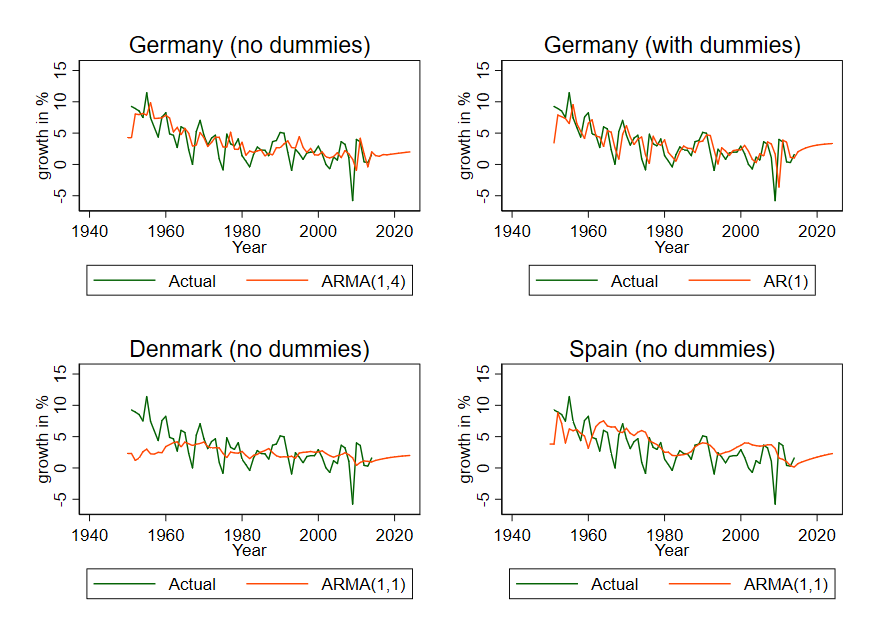
\includegraphics[width= \textwidth]{03_figures/fig23f}
  \label{fig:23f}
  \vspace{-1cm}
\end{figure}
